\section{Methods}

Each tag was represented as an ordered, fixed-length bitstring,
\begin{align*}
t = \langle t_0, t_1, t_2, \dots, t_{n-2}, t_{n-1} \rangle
\end{align*}
where
\begin{align*}
\forall i, t_i \in \{0, 1\}.
\end{align*}
In all experiments, we used 32 bit tags.

For consistency between metrics, we bound all metrics between 0 and 1.

\subsection{Integer Metric}

This metric is inspired by \citep{spector2011tag}.
They used positive integers between 0 and 100 to name referents.
Queries were provided the referent that had the next-larger value, wrapping around from 100 back to 0.

In this metric, we compare tags according to their value as an unsigned integer according to the following representation $f$,
\begin{align*}
f(t)
= \sum_{i=0}^{n-1} t_i \times 2^i.
\end{align*}

The distance metric $I$ between two length-$n$ tags $t$ and $u$ is
\begin{align*}
I(t, u) =
\begin{cases}
  \frac{2^n - f(t) + f(u)}{2^n}, & \text{if } f(t) > f(u), \\
  \frac{f(t) - f(u)}{2^n},         & \text{else} f(t) \leq f(u).
\end{cases}
\end{align*}

Note that this metric is non-commutative, i.e., it is not necessarily true that $I(t, u) = I(u, t)$.

Note also that this metric is one-dimensional.

A algorithmic advantage of this metric is that it allows for log-time matching.

\subsection{Hamming Metric}

This metric is based on the work of \citep{lalejini2019else}, originally after TODO hamming cite(?).

In this metric, we compare tags according to their bitwise hamming distance.
Mathematically speaking for tags $t$ and $u$ we compute the distance according to the metric $M$ as,
\begin{align*}
M(t, u)
= \frac{
  \#\{ i : t_i \neq u_i, i=0, \dots ,n-1\}
}{
  n
}
\end{align*}

This metric is commutative and $n$-dimensional.

\subsection{Hash Metric}

This metric is original to the our paper and meant to serve as a control.

The an arbitrary, but determinsitic value, uniformly distributed between 0 and 1.

We rely on the \texttt{hash\_combine} function, adapted from BOOST (TODO cite).

for two values \texttt{v1} and \texttt{v2}, \texttt{hash\_combine} is defined as follows
\begin{verbatim}
unsigned int hash_combine(
  unsigned int v1,
  unsigned int v2
) {
  return v1 ^ (
    v2 * 0x9e3779b9
    + (v1 << 6) + (v1 >> 2)
  );
}
\end{verbatim}

We compute the hash value of a tag as follows
\begin{verbatim}
unsigned int h(unsigned char *tag) {
  unsigned int result = tag[0];
  for (int i = 1; i < 4; ++i){
    result = hash_combine(result, t[i]);
  }
  return result;
}
\end{verbatim}
where \texttt{tag} is the tag's bitstring stored as an array of bytes.

To compute the metric $H$ we then call \texttt{hash\_combine} to combine the hash values of the tags $t$ and $u$
\begin{align*}
H(t, u) = \texttt{hash\_combine( h(}t\texttt{), h(}u\texttt{))}
\end{align*}

Note that this is not commutative.

\subsection{Streak Metric}

This metric was originally proposed by \citep{downing2015intelligence}.
Downing claims that it exhibits
It is computed according to the ratio between the longest contiguously matching substring among two bitsets and the longest contiguously mismatching substring among those two bitsets.
Downing claims that this metric exhibits greater robustness compared to integer and hamming distance metrics using mutational walk experiments but does not demonstrate it in an evolving system.

We define the greatest contiguously-matching length of $n$-long bitstrings $t$ and $u$ as follows,
\begin{align*}
m(t, u) = \max(\{i - j \forall i, j \in 0..n-1 \mid \forall q \in i..j, t_q = u_q \})
\end{align*}

We define the greatest contiguously-mismatching length as follows,
\begin{align*}
n(t, u) = \max(\{i - j \forall i, j \in 0..n-1 \mid \forall q \in i..j, t_q \neq u_q \})
\end{align*}

The streak metric $S'$  with tags $t$ and $u$
\begin{align*}
S'(t, u)
= \frac{ p(n(t,u)) }{p(m(t,u)) + p(n(t,u))}.
\end{align*}
where $p$ approximates the probability of a contiguously-matching substring between

It is worth noting that the formula for computing the probability of a $k$-bit match or mismatch, given by Downing as follows, is actually mathematically flawed.
\begin{align*}
p_k
= \frac{n - k + 1}{2^k}
\end{align*}

The probability of a $0$-bit match according to this formula would be computed as $p_0 = \frac{n - 0 + 1}{2^0} = n + 1$ which is clearly impossible because $p_0 > 1 \forall n > 0$.
The actual can probability be achieved using a lookup table computed using dynamic programming.

However, the formula Downing presented provides a useful approximation to the probability of a $k$ bit match.
For computational efficiency and consistency with the existing literature we use clamp edge cases between 0 and 1 to yield the corrected streak metric $S$.

\begin{align*}
S(t, u) =
\max( \min( S'(t, u), 1), 0)
\end{align*}

\subsection{Uniformification}

In experiments where actual match distance values, instead of the relative ranking of match distances, were mechanistically important or reported as data we transformed each match distance function such that the distribution of match distances of randomly generated bitstring pairs would approximate the uniform distribution between 0 and 1.
We sampled 10,000 randomly generated bitstring pairs to generate a set of match distances for each metric.
To generate a corrected distance for a raw distance $r$, we simply calculated its percentile ranking in the match distance database divided by one hundred.
If the exact raw distance $r$ wasn't present in the set of sampled match distances, we applied linear interpolation.
Specifically,
\begin{align*}
 p(m_b)/100.0 + r \times \frac{m_a - r}{m_a - m_b}
\end{align*}
where $p()$ is the percentile function, $m_a$ is the next-greater match distance, and $m_b$ is the next-lower match distance.

\begin{figure}
\begin{center}

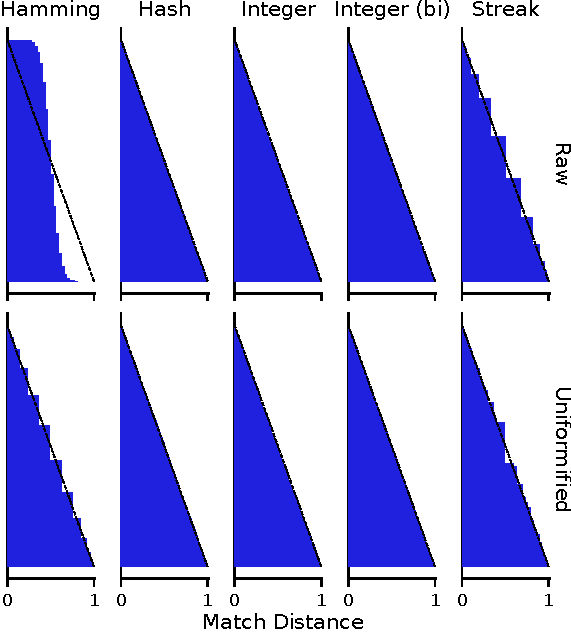
\includegraphics[width=\columnwidth]{img/uniformification/bitweight=0dot5+seed=1+title=low-score-distribution+_data_hathash_hash=75684cf1e73fb7f1+_script_fullcat_hash=d4b3b5e14a0d1350+ext=}
\caption{
Distance distributions of metrics before and after uniformification.
Dashed line indicates an ideal uniform distribution.
}
\label{fig:uniformification}

\end{center}
\end{figure}

Figure \ref{fig:uniformification} depicts the distributions of match distances between randomly sampled bitstring pairs for each metric before and after uniformification.

there's a lot of arbitrary metrics that could be created as follows
note that, for example,
\begin{align*}
f\Big( (0 \cup 1)^{32} \times (0 \cup 1)^{32} \Big) \rightarrow [0, 1]
\end{align*}

\begin{align*}
f^2\Big( (0 \cup 1)^{32} \times (0 \cup 1)^{32} \Big) \rightarrow [0, 1]
\end{align*}

What we're really interested is the ranking order of similarities over the $(0 \cup 1)^{32} \times (0 \cup 1)^{32}$ that the metric imposes, so applying a unifying transform onto the raw match distances helps to isolate that.
Plus, it provides an intuitive interpretation to match distances: a 0.01 distance match matches better than 99\% of all matches.

\subsection{Implementation}

We implemented our experimental system using the Empirical library for scientific software development in C++, available at \url{https://github.com/devosoft/Empirical}.
The code used to perform and analyze our experiments, our figures, data from our experiments, and a live in-browser demo of our system is available via the Open Science Framework at \url{https://osf.io/TODO/}.

% @AML: Just tacking this section on to the end of the Methods for now. It can get moved around/re-organized
%       as the rest of this paper takes shape.
\subsection{Tag-matching in a genetic programming context}

% - Lead-in text
%   - Overview of what we did
How does choice of tag-matching metric influence adaptive evolution in broader contexts?
We explore the implications of different tag-matching metrics in the context of SignalGP, a tag-based genetic
programming (GP) representation.
GP applies natural principles to evolve computer programs rather than writing them
by hand.
Spector et al. introduced tag-based naming in the context of GP (both linear and tree-based GP) as a
mechanism for associating evolvable names (tags) with program modules [citations].
SignalGP broadened the application of tag-based naming, using tags to enable signal-driven program
execution where tags specify the relationship between signals and signal-handlers (program modules)
[citation].

We investigate the success of five different tag-matching schemes (the integer, integer-symmetric, hash,
hamming, and streak metrics) in the context of SignalGP on two diagnostic GP problems: the changing-signal
task and the directional-signal task.
The changing-signal task evaluates how well a GP representation can associate
a set of distinct behavioral responses each with a particular environmental cue.
The directional-signal task evaluates how well a representation facilitates signal-response plasticity
(i.e., the ability to alter responses to repeated cues during the program's lifetime).

\subsubsection{SignalGP}

SignalGP (Signal-driven Genetic Programs) is a GP representation that enables signal-driven (i.e., event-driven)
program execution.
In SignalGP, programs are segmented into modules (function) that may be automatically triggered by
exogenously- or endogenously-generated signals.
Each module in SignalGP associates a tag (which can be used to reference the module) with a linear
sequence of instructions.
SignalGP makes explicit the concept of signals (events); signals comprise a tag and any signal-specific
data.
Because both program modules and signals have associated tags, SignalGP uses tag-based referencing to
determine the most appropriate module to trigger in response to a signal.
Signals trigger the module with the closest matching tag (according to a given tag-matching metric),
using any signal-associated data as input to the triggered module.
SignalGP can handle many signals simultaneously, processing each in parallel.

% @AML: some of this paragraph is too similar to the one in the genetic regulation paper. Needs to be
%       adjusted accordingly in future editing iterations.
The SignalGP instruction set, in addition to including traditional computational operations, allows
programs to generate internal signals, broadcast external signals, and otherwise work in a tag-based context.
Instructions contain arguments, which include an evolvable tag; arguments may modify the effect of an
instruction, often specifying memory locations or fixed values.
For example, instructions may refer to program modules using tag-based referencing, and when an instruction
generates a signal (e.g., to be used internally or broadcast), the instruction's tag specifies the signal's
tag.
Additionally, SignalGP supports genetic regulation with promoter and repressor instructions
that, when executed, allow programs to adjust how well subsequent signals match with a target function
(targets are determined using instruction tags).
We describe the full SignalGP instruction set used in this work in [SignalGP supplemental material].
For a more detailed description of SignalGP, see [citation].

\subsubsection{Changing-signal Task}

% - Diagnostic Tasks
%   - Changing signal task
%     - experiment
%   - Directional signal task
%     - experiment

\subsubsection{Directional-signal Task}
